
\chapter{一般化ムーアグラフ}
\label{chap:generalized-moore-graph}
本章では一般化ムーアグラフを定義する.さらに,一般化ムーアグラフが満たす
いくつかの性質を示す.
\begin{definition}[Cerfら\cite{Cerf1973}]\rm
  \label{def:generalized-moore-graph}
  次の性質が成り立つ頂点数$n$,次数$k$の正則グラフを
  \textbf{一般化ムーアグラフ}(\textbf{Generalized Moore graph})とよぶ.

  すべての頂点$v$について,$v$との距離が$i$である頂点の数$c_i$が,
  \begin{equation}
    \label{eq:gmg-verts-dist}
    \begin{aligned}
      c_i =
      \begin{cases}
        k(k-1)^{i-1} & 1\leq i\leq Q \\
        R & i = Q+1 \\
        0 & Q+2\leq i \leq n-1
      \end{cases}
    \end{aligned}
  \end{equation}
  を満たすこと.ただし,
  \begin{align}
    Q(n,k)&=\max\{q|n-1-\sum_{i=1}^{q}k(k-1)^{i-1}\geq 0\}\label{eq:gmg-q} \\
    R(n,k)&=n-1-\sum_{i=1}^{Q(n,k)}k(k-1)^{i-1}\label{eq:gmg-r}
  \end{align}
  とする.
\end{definition}
\begin{example}\rm
  図\ref{fig:gmg-example}に頂点数と次数がそれぞれ12と3の一般化ムーアグラフの例を示す.
  $Q(12,3)$と$R(12,3)$はそれぞれ,
  \begin{align*}
    Q(12,3) &= \max\{q | 12-1-\sum_{i=1}^{q}3\cdot2^{i-1} \geq 0\} = 2 \\
    R(12,3) &= 12 - 1 - \sum_{i=1}^{Q(12,3)}3\cdot2^{i-1} = 2
  \end{align*}
  である.このグラフの頂点$1$に着目すると,距離が$i$の頂点数$c_i$は,
  \begin{align*}
    c_1&= |\{2,3,4\}| = 3 = 3\cdot2^0 & \\
    c_2&= |\{5,6,7,8,9,10\}| = 6 = 3\cdot2^1 & \\
    c_3&= |\{11,12\}| = 2 = R(12,3) & \\
    c_i&= 0 & (i>3)
  \end{align*}
  となるので,式\ref{eq:gmg-verts-dist}で示した距離と頂点数の
  関係を満たす.同様に,他のすべての頂点について,同様の距離と頂点数の関係を
  満たす.
  \begin{figure}
    \centering
    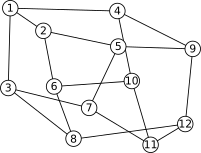
\includegraphics{gmg-example.pdf}
    \caption{頂点数12,次数3の一般化ムーアグラフの例}
    \label{fig:gmg-example}
  \end{figure}
\end{example}
以下,頂点数$n$,次数$k$の一般化ムーアグラフを$M(n,k)$と記す.
$Q(n,k)$と$R(n,k)$をそれぞれ式\ref{eq:gmg-q}と式\ref{eq:gmg-r}のとおりとする.
$M(n,k)$と$Q(n,k)$と$R(n,k)$について,
頂点数と次数が文脈から明らかな場合は省略してそれぞれ$M,Q,R$と表す.

一般化ムーアグラフの頂点間距離の総和を求め,これが正則グラフの頂点間距離の総和の
下界であることを示す.
\begin{theorem}[Cerfら\cite{Cerf1974Lower}]\rm
  \label{thm:gmg-lower-bound}
  $M(n,k)$の頂点間距離の総和は,
  \begin{equation}
    \label{eq:gmg-lb}
    S(n,k) = \sum_{(s,t)\in V\times V}d(s,t) =
    n \left[\ \sum^{Q}_{i=1}ik(k-1)^{i-1} + (Q+1)R\ \right]
  \end{equation}
  で与えられる.これは,頂点数が$n$,次数が$k$の正則グラフの頂点間距離の総和の下界である.
\end{theorem}
\begin{proof}\rm
  ある頂点$v$から頂点$w(\neq v)$との距離の総和を次式で表す.
  \begin{equation}
    \label{eq:gmg-lb-1}
    \sum_{i=1}^{n-1}i c_i
  \end{equation}
  ここで,$c_i$は$v$との距離が$i$の頂点の個数とする.
  一般化ムーアグラフの場合,$c_i$は式\ref{eq:gmg-verts-dist}で与えられる.
  そのため,式\ref{eq:gmg-lb-1}から,
  \begin{align}
      \sum_{i=1}^{n-1}ic_i
      &=\sum_{i=1}^{Q}ic_i+(Q+1)c_{Q+1}+\sum_{i=Q+2}^{n-1}ic_i \nonumber\\
      &=\sum_{i=1}^{Q}ik(k-1)^{i-1}+(Q+1)R
      \label{eq:gmg-lb-2}
  \end{align}
  が得られる.これは一つの頂点から他のすべての頂点への距離の総和を表すので,
  式\ref{eq:gmg-lb-2}を$n$倍すると,式\ref{eq:gmg-lb}が得られる.

  次に,式\ref{eq:gmg-lb}が頂点数が$n$,次数が$k$の正則グラフの頂点間距離の総和の
  下界であることを示す.一般的な$c'_i$に対して,
  \begin{equation}
    \label{eq:gmg-lb-3}
    \sum_{i=1}^{n-1}i c_i \leq \sum_{i=1}^{n-1}i c'_i
  \end{equation}
  であることを証明する.
  $1\leq i\leq Q$の範囲で,$c_i$は最大なので次が得られる.
  \begin{equation}
    \label{eq:gmg-lb-4}
    \begin{aligned}
      c_i - c'_i
      \begin{cases}
        \geq 0 & 1\leq i\leq Q \\
        \lesseqgtr 0 & i = Q+1 \\
        \leq 0 & Q+2\leq i\leq n-1
      \end{cases}
    \end{aligned}
  \end{equation}
  $c_{Q+1}\geq c'_{Q+1}$と$c_{Q+1}\leq c'_{Q+1}$のふたつの場合について考える.
  $c_{Q+1}\geq c'_{Q+1}$のとき,
  $c_{Q+1}\geq c'_{Q+1}$ならば$c_{Q+1}-c'_{Q+1}\geq0$となり,
  式\ref{eq:gmg-lb-4}より,
  \begin{equation}
    \label{eq:gmg-lb-5a}
    \begin{aligned}
      c_i-c'_i
      \begin{cases}
        \geq 0 & 1\leq i\leq Q+1 \\
        \leq 0 & Q+2\leq i\leq n-1
      \end{cases}
    \end{aligned}
  \end{equation}
  が成り立つ.$c_i$の定義より,次が成り立つ.
  \begin{equation}
    \label{eq:gmg-lb-6}
    \sum_{i=1}^{n-1}c_i = \sum_{i=1}^{n-1}c'_i = n-1
  \end{equation}
  式\ref{eq:gmg-lb-5a}と式\ref{eq:gmg-lb-6}より,
  \begin{equation}
    \label{eq:gmg-lb-7a}
    \begin{aligned}
      \sum_{i=1}^{Q+1}(c_i-c'_i) &= \sum_{i=1}^{Q+1}|c_i-c'_i| \\
      \sum_{i=Q+2}^{n-1}(c_i-c'_i) &= -\sum_{i=Q+2}^{n-1}|c_i-c'_i| \\
      \sum_{i=1}^{Q+1}|c_i-c'_i| &= \sum_{i=Q+2}^{n-1}|c_i-c'_i|
    \end{aligned}
  \end{equation}
  が得られる.式\ref{eq:gmg-lb-7a}を用いて,式\ref{eq:gmg-lb-8a}を考える.
  \begin{equation}
    \label{eq:gmg-lb-8a}
    \sum_{i=1}^{n-1}i(c_i-c'_i)=
    \sum_{i=1}^{Q+1}i|c_i-c'_i|-\sum_{i=Q+2}^{n-1}|c_i-c'_i|
  \end{equation}
  式\ref{eq:gmg-lb-8a}の第一項の上界は,式\ref{eq:gmg-lb-8a1}である.
  \begin{equation}
    \label{eq:gmg-lb-8a1}
    \sum_{i=1}^{Q+1}i|c_i-c'_i|\leq (Q+1)\sum_{i=1}^{Q+1}|c_i-c'_i|
  \end{equation}
  式\ref{eq:gmg-lb-8a}の第二項の下界は,式\ref{eq:gmg-lb-8a2}である.
  \begin{equation}
    \label{eq:gmg-lb-8a2}
    \sum_{i=Q+2}^{n-1}i|c_i-c'_i|\geq (Q+2)\sum_{i=Q+2}^{n-1}|c_i-c'_i|
  \end{equation}
  式\ref{eq:gmg-lb-8a1}と式\ref{eq:gmg-lb-8a2}より,次が成り立つ.
  \begin{align*}
    \sum_{i=1}^{n-1}i(c_i-c'_i)
    &\leq (Q+1)\sum_{i=1}^{Q+1}|c_i-c'_i|-(Q+2)\sum_{i=Q+2}^{n-1}|c_i-c'_i| \\
    &= (Q+1)\sum_{i=1}^{Q+1}|c_i-c'_i|-(Q+2)\sum_{i=1}^{Q+1}|c_i-c'_i| \\
    &= -\sum_{i=1}^{Q+1}|c_i-c'_i| \\
    &\leq 0
  \end{align*}
  ゆえに式\ref{eq:gmg-lb-3}が成り立つ.
  $c_{Q+1}\leq c'_{Q+1}$の場合も,総和の範囲が異なることを除いて同じである.
\end{proof}

次の性質は,一般化ムーアグラフが満たす構造的な性質を示す.
後に説明する探索方法に用いる重要な性質である.
\begin{theorem}\rm
  \label{thm:gmg-geometric-property}
  ある正則グラフが一般化ムーアグラフであることの必要十分条件は,
  \begin{enumerate}[(a)]
  \item 長さ$2Q$以下の閉路を持たないこと
    \label{gmg-geom-a}
  \item $R=0$のとき,直径が$Q$,\hspace{2ex}$R>0$のとき,直径が$Q+1$であること.
    \label{gmg-geom-b}
  \end{enumerate}
  の二条件を同時に満たすことである.
\end{theorem}
\begin{proof}\rm
  正則グラフの頂点数を$n$,次数を$k$とする.
  条件(\ref{gmg-geom-a})を満たすならば,すべての頂点$v$に対して,
  $d(v,w)=i$なる頂点$w$の数$c'_i$は,$c'_i=k(k-1)^{i-1}(1\leq i\leq Q)$となる.
  また,条件(\ref{gmg-geom-b})を満たすならば,$c'_i=0(Q+2\leq i)$である.
  これら二つを同時に満たすとき,
  \[ c'_{Q+1}=n-1-\sum_{i=1}^{Q}k(k-1)^{i-1}=R \]
  を満たす.よって,ある正則グラフが条件(\ref{gmg-geom-a})と
  条件(\ref{gmg-geom-b})を同時に満たすとき,それは$M(n,k)$である.

  逆を証明する.$c_i=k(k-1)^{i-1}(1\leq i\leq Q)$なので,
  すべての頂点$v$について,頂点$w\,(d(v,w)=i<Q)$は
  $k-1$個の頂点$x\,(d(v,x)=i+1)$と隣接する.
  従って,一般化ムーアグラフ$M(n,k)$には,長さ$2Q$以下の閉路は存在しない.
  直径について議論する.$R=0$の場合,$Q+1\leq i$を満たす$i$について,$c_i=0$なので,
  すべての頂点$v$について,$d(v,w)\geq Q+1$となるような頂点$w$は存在しない.従って
  直径は$Q$である.$R>0$の場合も同様に,$Q+2\leq i$を満たす$i$について$c_i=0$なので,
  すべての頂点$v$について,$d(v,w)\geq Q+2$となるような頂点$w$は存在しない.従って
  直径は$Q+1$である.以上から,$M(n,k)$は条件(\ref{gmg-geom-a})と
  条件(\ref{gmg-geom-b})を同時に満たす.
\end{proof}
便宜上,$M(n,k)$の直径を$\hat{Q}(n,k)$または$\hat{Q}(n)$,$\hat{Q}$で表す.
$\hat{Q}(n)$は,最大次数$k$の平衡木において,頂点$1$から順に,頂点$1$から遠くなるように並べた
ときの$1$と$n$との距離に等しいことに注意する.最大次数$k$の平衡木を
図\ref{fig:balanced-tree}に示す.
\begin{figure}
  \centering
  \def\svgwidth{.4\textwidth}
  \input{balanced-tree.pdf_tex}
  \caption{最大次数$k$の平衡木の例}
  \label{fig:balanced-tree}
\end{figure}

